\documentclass[conference]{IEEEtran}
\IEEEoverridecommandlockouts
% The preceding line is only needed to identify funding in the first footnote. If that is unneeded, please comment it out.
\usepackage{cite}
\usepackage{amsmath,amssymb,amsfonts}
\usepackage{algorithmic}
\usepackage{textcomp}
\usepackage{xcolor}
\usepackage{graphicx}
\graphicspath{ {./images/} }
\def\BibTeX{{\rm B\kern-.05em{\sc i\kern-.025em b}\kern-.08em
    T\kern-.1667em\lower.7ex\hbox{E}\kern-.125emX}}
\begin{document}

\title{Report of "Image Source Identification" project*\\
{\footnotesize Master's degree in Artificial Intelligence Systems\newline
Trends and Applications of Computer Vision; A.Y 2022/2023\newline 
Cecilia Pasquini, Zhun Zhong\newline}
}

\author{\IEEEauthorblockN{Joy Battocchio}

\and
\IEEEauthorblockN{Davide Guidolin}

\and
\IEEEauthorblockN{Alessio Belli}

\and
\IEEEauthorblockN{Alberto Casagrande}
% \IEEEauthorblockA{\textit{dept. name of organization (of Aff.)} \\
% \textit{name of organization (of Aff.)}\\
% City, Country \\
% email address or ORCID}
}

\maketitle

\section{Introduction}
Source identification is one of the most important tasks in digital image forensics. 
In fact, the ability to reliably associate an image with its acquisition device may be crucial both during investigations and before a court of law.
The key assumption of forensics source identification is that acquisition devices leave traces in the acquired content, and that instances of these traces are specific to the respective (class of) device(s). 
This kind of traces is present in the so-called device fingerprint.
A major impulse to research in this field came with the seminal work of Lukas et al. showing that reliable device identification is possible based on the camera photo-response non uniformity (PRNU) pattern. 
%This is a multiplicative noise component caused by the inhomogeneity of silicon wafers and imperfections of the sensor manufacturing, which, in turn, cause a non-uniform sensitivity to light among the sensor photo-diodes. 
%This means that a pixel could be slightly brighter or darker than expected by camera design, and each pixel is individually affected by this issue. 
Each camera is characterized by its unique PRNU pattern, which can be regarded as a sort of camera fingerprint.
All photos taken by a given camera carry traces of its fingerprint which, under suitable hypotheses, can be retrieved, enabling reliable device identification and brand and model identification as well.
%In order to compose your camera fingerprint, the best possible scenario and condition is flat images of blue or cloudy sky.
However, due to spatial transformations, filtering, AI post-processing and more in general in-device or out-device post-processing, PRNU is today more than ever compromised. 
Even for media coming from the exact same device, it is really difficult that we can compare the two PRNUs of these ones straightforwardly, but we need to resynchronize one with respect to the other.
In fact, Mandelli et al.'s work is based on the assumption that the images are already geometrically synchronized.
Its main contribution is using a 2 channel CNN network that for every device d $\in$ DT is fed using noise residuals coming from device d, paired with PRNU K$_{d}$ (coherent pair) and with PRNU K$_{d}^{-}$ coming from a different device (non-coherent pair). 
The CNN is able to learn a similarity measure Cs for the source identification task.
This method proves to be generally faster than PCE, in particular when a large amount of potential provenance devices is investigated, requiring much less query image content to obtain enhanced attribution accuracy.



\section{Related works}Of all the related works cited in the main paper, it has been decided to focus on three:
\begin{itemize}
    \item \textbf{Kharrazi et al.} "Blind source camera identification"\cite{Kharrazi}
    \item \textbf{Lukáš et al.} "Digital camera identification from sensor pattern noise"\cite{Lukas}
    \item \textbf{Bondi et al.} "First Steps Toward Camera Model Identification with Convolutional Neural Networks"\cite{Bondi}
\end{itemize}
The choice is motivated by the influence that these three works had on the Mandelli's one.
They all represent important milestones in the solution of the source identification problem.
For this reason it has been decided to present them in temporal order of publication, because each one of them gives an additional contribution and it's logically dependent on the previous ones.

\subsection{Kharrazi et al.}
The authors of "Blind source camera identification" propose to extract handcrafted features from images in order to use them as input for a SVM classifier.
\\The chosed features are the ones that bring more evidence of the CFA configuration and the color processing carried out by the camera, which should be unique for each sensor and therefore useful for their identification.
\\In particular they are:
\begin{itemize}
    \item \textbf{Average pixel value}. Average values in RGB channels of an image should average to gray assuming that the images has enough color variations.
    \item \textbf{RGB pairs correlation}. Capture the fact that depending on the camera structure, the correlation between different color bands could varies.
    \item \textbf{Neighbor distribution Center of mass}. Calculating the number of pixel neighbors for each pixel value, where the pixel neighbors are defined as all pixels having a difference in value of 1 or -1, from the pixel value in question. This is calculated for each color band.
    \item \textbf{RGB pairs energy ratio}. It is used in the process of white point correction.
    \item \textbf{Wavelet domain statistic}. Decompose each color band of the image using separable quadratic mirror filters and then calculate the mean for each of the 3 resulting sub-bands.
\end{itemize}
In addition to these features, different cameras produce images of different quality, so we can extract the Image Quality Metrics as features to aid in distinguishing between cameras. 
These metrics are:
\begin{itemize}
    \item \textbf{Pixel difference based measures}. Mean squared error, mean absolute error, ...
    \item \textbf{Correlation based measures}. Normalized cross correlation, ...
    \item \textbf{Spectral distance based measures}. Spectral phase and magnitude errors.
\end{itemize}
As it is written above, these features are then used by a SVM to classify the right source camera.
\textcolor{red}{insert cons??}
\subsection{Lukáš et al.}
In the paper "Digital camera identification from sensor pattern noise" the authors proposed a new method for the camera identification problem that is based on the sensor's pattern noise. 
The basic idea is to compute for each camera a pattern noise that can act as a unique fingerprint. Then, if you want to identify the camera that shoot a specific photo, the paper suggests to use a correlation filter in order to compare the noise residual of the image with the fingerprint of all the cameras inside the dataset.

In the image acquisition process, there are many sources of imperfections and noise that can enter into various phases. Among these noises, we can identify two types of noise: \textit{shot noise} (a random component) and \textit{pattern noise}. The latter is a deterministic component that has the characteristic of remaining approximately the same if different images of the same scene are taken. This is why this type of noise can be used for the camera identification problem.\subsection{Bondi et al.}
About 10 years after the PRNU-based method for digital camera identification, in 2017, the authors of "First Steps Toward Camera Model Identification with Convolutional Neural Networks" investigated a novel approach to solve the camera model identification problem, based on Convolutional Neural Networks. The choice was fully motivated by other successful deep-learning algorithms applied to forensics tasks.
In particular, they made use of a \textit{Convolutional Neural Network} (CNN) which learns the features characterizing each camera model directly from the acquired images, rather than using handcrafted features. In addition, they also used linear \textit{Support Vector Machines} (SVMs) for classification.

The training and evaluaton pipelines are shown in figure ...

Given a set of training and validation labeled samples coming from \textit{N} known camera models, the training proceeds as follows:
for each image \textit{I} with the corresponding label \textit{L} (camera model), \textit{K} non overlapping patches are extracted, where each patch \textit{P\textsubscript{k}} inherits the same label \textit{L} of the source image. For each patch, the CNN extracts a feature vector \textit{V\textsubscript{k}} of 128 elements. The resulting feature vectors are then used to train a battery of $ N \cdot (N - 1)/2 $ linear binary SVM classifiers \textit{S}. 
During evaluation, the battery \textit{S} of linear SVMs assigns a label $\hat{L}$\textit{\textsubscript{k}} to each patch. The predicted label $\hat{L}$ for image \textit{I} is obtained through majority voting on $\hat{L}$\textit{\textsubscript{k}}, $k \in [1, K]$.

The advantages of the proposed CNN are mainly two:
\begin{itemize}
	\item It learns a feature extraction methodology that generalizes well on a set of unknown camera models;
	\item The resulting feature vectors have only 128 elements, allowing to characterize camera models in a space with reduced dimensionality and  consequently enabling the use of simple classifiers like SVMs.
\end{itemize}


\input{related_works}


\section{CNN-based fast source device identification}
\begin{figure}[t!]
    \centering
    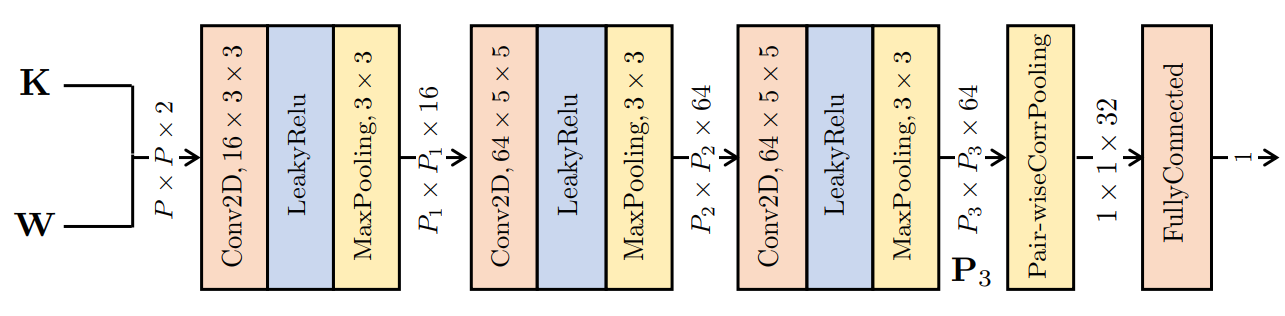
\includegraphics[keepaspectratio, width=0.5\textwidth]{CNN_architecture}
    \caption{Pair-Wise Correlation Network (PCN) architecture}
    \label{fig:CNN_architecture}
\end{figure}

We were assigned the paper \textit{CNN-based fast source device identification}\ref{AA} by, \textit{Mandelli et al.}

In this paper the authors propose a CNN-based approach to address the problem of source device identification based on PRNU. 
In particular, their goal is to replace the PCE test with an alternative method based on CNN. Their approach differs from the one
proposed by Bondi et al. because they train an end-to-end network instead of using a CNN to produce features used by an SVM.

The core idea of this paper is to use a 2-channel CNN to compare the estimated device PRNU $K_d$ with the noise residual $W$ 
obtained from the given test image $I$.

First of all they estimate the device PRNU $K_d$ [2] from a set of flat-field images taken from the same device and they extract the
noise residual $W$ from a set of images depicting natural scenes.
Then they crop the central $P$x$P$ pixel region from both $K_d$ and $W$ and they feed the CNN with these 2 image patches.
Since the method is independent from the used CNN they experiment different pre-trained networks and they propose a simple but 
effective architecture that is composed of 3 convolutional layers, a pair-wise correlation pooling layer and a fully connected 
layer (Fig. \ref{fig:CNN_architecture}). The pair-wise correlation pooling layer computes the correlation between adjacent pairs of features, while the
fully connected layer outputs an identification score $C_s$ that is high for coherent pairs and low for non-coherent ones. 

The network can be used in both a closed-set scenario and in an open-set scenario. In the closed-set scenario we have a finite set 
of devices and we have to identify the source of the image from that set. In the open-set scenario we have a test image and a candidate
device and we have to tell if that device shot the given image.

The authors shows that in both the open and closed set scenario the proposed approach outperforms the PCE test both in accuracy 
and inference time. In particular, regarding the closed set scenario, we can see from (Fig 2) that the proposed Pair-wise Correlation Net (PCN) is faster than all the 
other architectures and it outperforms PCE in accuracy, however it is outperformed by the other networks. It is important to notice 
also that all the methods perform better when the patch size is bigger.
Regarding the open set scenario, the area under the ROC curve related to the patch size is shown in (Fig 3) and it's clear that 
PCE is worst than all proposed architectures. 
Finally, in (Fig 4), we can see the accuracy as a function of crop size when the dataset is double-JPEG compressed. The PCN outperforms
PCE even after double compression and we can notice that the performances are better when both the PRNU and the noise residual are 
extracted from double compressed images.

\input{paper}

\begin{thebibliography}{00}
\bibitem{Kharrazi} M. Kharrazi, H. T. Sencar and N. Memon, "Blind source camera identification," 2004 International Conference on Image Processing, 2004.
\bibitem{Lukas} J. Lukas, J. Fridrich, and M. Goljan, “Digital camera identification from sensor pattern noise”.
\bibitem{Bondi} L. Bondi, L. Baroffio, D. Guera, P. Bestagini, E. Delp, and S. Tubaro , "First Steps Toward Camera Model Identification with Convolutional Neural Networks".
\bibitem{Mandelli} S. Mandelli, D. Cozzolino, P. Bestagini, L. Verdoliva and S. Tubaro, "CNN-Based Fast Source Device Identification"
\end{thebibliography}
\vspace{12pt}
\end{document}
